% ============================================================
% Game Design Documentation — 主文件（Master File）
% 编译方式（在本目录下）：
%   pdflatex main.tex   （连续跑 2~3 次，让目录/图号/引用稳定）
% 或一次性：latexmk -pdf main.tex
% ------------------------------------------------------------
% 结构：
%   chapters/01_game_core.tex         ~/07_version.tex   章节子文件
%   chapters/Appendix/*.tex                               附录子文件
%   figures/Chapter*/                 图片（按章节归类）
% 合并原理：\include{chapters/xxx} 会把子文件内容合并进本文档，
%           编译一次 main.tex 即得到完整 PDF。
% ============================================================
\documentclass[11pt]{article}

\usepackage[a4paper,margin=1in]{geometry}   % A4 纸张（中国通用），1 英寸页边距
\usepackage{amsmath,amssymb}
\usepackage{graphicx}
\usepackage{booktabs}
\usepackage{enumitem}
\usepackage{microtype}
\usepackage{setspace}
\usepackage{newtxtext,newtxmath}   % Times New Roman 风格字体（正文+数学）
\usepackage[colorlinks=true,linkcolor=blue,urlcolor=blue]{hyperref}
\usepackage[edges]{forest}
\usepackage{seqsplit}   % 长路径断行：允许在任意字符处换行，防止溢出纸外

% 全局 1.5 倍行距
\onehalfspacing

% 图片目录（按章节分文件夹，全部注册到这里，正文只需写文件名）
\graphicspath{{figures/Chapter00_Cover/}{figures/Chapter03_Player/}{figures/Chapter04_FogOfWar/}{figures/Chapter05_RandomDungeonMap/}}

% 反斜杠快捷命令（用于文档中的 Windows 路径）
% \hspace{0pt} 是"零宽可断行点"：让长路径可以在每个反斜杠处自动换行，
% 不会再把文字挤到纸外。所有用 \bs 的路径都自动受益。
\newcommand{\bs}{\textbackslash\hspace{0pt}}

% 封面标题：
%   \emph{...}                             → 斜体
%   \fontsize{字号pt}{行距pt}\selectfont  → 精确控制字号（30pt 比默认标题 \Huge 的 24.88pt 大一档）
%   \\[1.2em]                              → 换行并空出一行高度（主标题与副标题之间）
%   \Large                                → 游戏名 Monster Dungeon 用 \Large（比 \large 大一级）
\title{\emph{\fontsize{30pt}{36pt}\selectfont Game Design Documentation}\\[1.2em]\fontsize{30pt}{36pt} Monster Dungeon}
\author{}
\date{Version 1.2}

\begin{document}

\maketitle

% 封面图（不编号）
\begin{center}
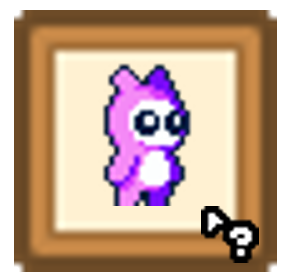
\includegraphics[width=0.8\textwidth]{cover.png}
\end{center}
\thispagestyle{empty}   % 封面页不显示页码
\clearpage

% 目录独立成页：封面结束后另起新页，目录结束后也另起新页进正文
% 目录本身用单倍行距+小字号，保证一页装下（正文保持 1.5 倍行距）
{\small
\begin{singlespace}
\tableofcontents
\end{singlespace}}
\thispagestyle{empty}   % 目录页不显示页码
\clearpage

\setcounter{page}{1}    % 正文页码从 1 重新开始

% !TeX root = ../main.tex
% ============================================================
% Chapter 1: Game Core
% 说明：本文件由 main.tex 通过 % !TeX root = ../main.tex
% ============================================================
% Chapter 1: Game Core
% 说明：本文件由 main.tex 通过 % !TeX root = ../main.tex
% ============================================================
% Chapter 1: Game Core
% 说明：本文件由 main.tex 通过 \include{chapters/01_game_core} 合并进主文档。
%       章节编号由 LaTeX 自动生成，请勿手工编号。
%       内容忠实来自 策划案.docx 原文（英文），未做改写。
% ============================================================
\section{Game Core}

This is a dungeon level-up game. The player collects what they need to clear each level, and the final goal is to defeat the Boss.

\subsection{The Most Significant Design in the Game}

Before reading this chapter, let's think about what makes a game fun and keeps players playing. A fun game comes from these things:

\begin{enumerate}
  \item The Core: Decision.
  \item The heartbeat around the core: Uncertainty.
  \item The decoration of the decision: the density of decisions and their consequences.
\end{enumerate}

A fun game is packed with interesting decisions. The character, eye-catching visuals, and UI are the decoration around those decisions.

The decisions serve the core loop: beat enemies, feel your growth, and take on challenges that never seem to end.

\subsection{The Core Design Applied in My Game}

The game has several systems: Player, Fog of War, Task, Random Dungeon, Enemy, and more.

First, Decision: the core loop is that the player collects equipment, enters the dungeon, defeats enemies, reaches the exit portal, and chooses to extract or enter the next, harder level. The player's final goal is to defeat the Boss.

Second, Uncertainty: to create uncertainty, I added a Fog of War system and used an algorithm to generate the random dungeon map.

Third, the decoration: to make decisions more interesting, I added the Task System, wrote some story, and designed various weapons, monsters, and chest loot, giving players more choices. I also optimized the dungeon generation algorithm to make maps more balanced and create more decision points in combat.
 合并进主文档。
%       章节编号由 LaTeX 自动生成，请勿手工编号。
%       内容忠实来自 策划案.docx 原文（英文），未做改写。
% ============================================================
\section{Game Core}

This is a dungeon level-up game. The player collects what they need to clear each level, and the final goal is to defeat the Boss.

\subsection{The Most Significant Design in the Game}

Before reading this chapter, let's think about what makes a game fun and keeps players playing. A fun game comes from these things:

\begin{enumerate}
  \item The Core: Decision.
  \item The heartbeat around the core: Uncertainty.
  \item The decoration of the decision: the density of decisions and their consequences.
\end{enumerate}

A fun game is packed with interesting decisions. The character, eye-catching visuals, and UI are the decoration around those decisions.

The decisions serve the core loop: beat enemies, feel your growth, and take on challenges that never seem to end.

\subsection{The Core Design Applied in My Game}

The game has several systems: Player, Fog of War, Task, Random Dungeon, Enemy, and more.

First, Decision: the core loop is that the player collects equipment, enters the dungeon, defeats enemies, reaches the exit portal, and chooses to extract or enter the next, harder level. The player's final goal is to defeat the Boss.

Second, Uncertainty: to create uncertainty, I added a Fog of War system and used an algorithm to generate the random dungeon map.

Third, the decoration: to make decisions more interesting, I added the Task System, wrote some story, and designed various weapons, monsters, and chest loot, giving players more choices. I also optimized the dungeon generation algorithm to make maps more balanced and create more decision points in combat.
 合并进主文档。
%       章节编号由 LaTeX 自动生成，请勿手工编号。
%       内容忠实来自 策划案.docx 原文（英文），未做改写。
% ============================================================
\section{Game Core}

This is a dungeon level-up game. The player collects what they need to clear each level, and the final goal is to defeat the Boss.

\subsection{The Most Significant Design in the Game}

Before reading this chapter, let's think about what makes a game fun and keeps players playing. A fun game comes from these things:

\begin{enumerate}
  \item The Core: Decision.
  \item The heartbeat around the core: Uncertainty.
  \item The decoration of the decision: the density of decisions and their consequences.
\end{enumerate}

A fun game is packed with interesting decisions. The character, eye-catching visuals, and UI are the decoration around those decisions.

The decisions serve the core loop: beat enemies, feel your growth, and take on challenges that never seem to end.

\subsection{The Core Design Applied in My Game}

The game has several systems: Player, Fog of War, Task, Random Dungeon, Enemy, and more.

First, Decision: the core loop is that the player collects equipment, enters the dungeon, defeats enemies, reaches the exit portal, and chooses to extract or enter the next, harder level. The player's final goal is to defeat the Boss.

Second, Uncertainty: to create uncertainty, I added a Fog of War system and used an algorithm to generate the random dungeon map.

Third, the decoration: to make decisions more interesting, I added the Task System, wrote some story, and designed various weapons, monsters, and chest loot, giving players more choices. I also optimized the dungeon generation algorithm to make maps more balanced and create more decision points in combat.

% !TeX root = ../main.tex
% ============================================================
% Chapter 2: Game Program Structure
% 说明：本文件由 main.tex 合并进主文档。章节编号 LaTeX 自动生成。
%       内容忠实来自 策划案.docx 原文（英文）。
%       % TODO: 标记的小节是原文只有标题、没有内容的部分（待补充索引）。
% ============================================================
\section{Game Program Structure}

The game uses a message bus + Game Message to decouple its systems. Each system manages its own scripts. One system handles one object type, and one script handles one function. Different systems connect through the message bus.

Before this structure, I tried a Game Manager / Director pattern to control the whole game system, but it lost the battle: different functions became coupled together. Then I combined the Game Manager with a state machine and a message bus to organize the code. But this defect surfaced as the code grew past about 13k lines. The Game Manager and the state machine could be separated into one independent system that publishes the game state. At September 30, 2026, I completed the new code structure.

\begin{quote}
\emph{Designer Note:}
\end{quote}

\subsection{Message Bus + Game Message \& Field Distribution}

The Message Bus + Game Message base class system send messages and completed data for different systems or fields, different fields owns different message bus and The Supreme Message Bus manages messages among different fields.

Distribute functions into these fields: Game State, Player, Enemy, Item, Inventory, World and independent function module names `Execution \& Static Scripts'.

\subsection{Ports}

\begin{enumerate}
  \item Directly Quote: In modules, deal with massive data with high speed.
  \item Message Bus: Event Communication that publish significant events.
  \item Shared Data: modules one another with massive data communications.
\end{enumerate}

\subsection{Game State}

\begin{enumerate}
  \item Communication: Only Message Bus.
  \item Responsibility: Declare the Game State
  \item State types: Main World, Dungeon + Layer.
  \item % TODO: 原文第 4 点为空，待补充
\end{enumerate}

\subsection{Player}
% TODO: 原文仅有标题，内容待补充

\subsection{Enemy}
% TODO: 原文仅有标题，内容待补充

\subsection{Item}
% TODO: 原文仅有标题，内容待补充

\subsection{Inventory}
% TODO: 原文仅有标题，内容待补充

\subsection{World}
% TODO: 原文仅有标题，内容待补充

% !TeX root = ../main.tex
% ============================================================
% Chapter 3: Player
% 说明：本文件由 main.tex 合并进主文档。章节编号 LaTeX 自动生成。
%       内容忠实来自 策划案.docx 原文（英文）。
%       路径中的反斜杠用 \bs （在 main.tex 中定义为 \textbackslash）。
%       % TODO: 标记的小节是原文只有标题、没有内容的部分（待补充索引）。
% ============================================================
\section{Player}

\subsection{Module Description}

\begin{enumerate}
	\item Player Config: Store the player's initialization config file.
	\item Player Attack: Properties: Control the player attack mode. Describe at \ref{PlayerAttack}.
	\item Player Health: Properties: Control the player health. Descibe at \ref{PlayerHealth}.
	\item Player Movement: Properties: Control the player movement. Describe at \ref{PlayerMovement}.
	\item Player Stamina: Properties: Control the player stamina. Describe at \ref{PlayerStamina}.
\end{enumerate}

\subsection{System Pipeline}

\begin{enumerate}
	\item Keyboard input detection: Control the player's movement and summon the functions.
	\item Properties: Player Renderer, Player Attack, Player Movement, Player Stamina.
\end{enumerate}

\subsection{SubModule Pipeline}

\subsubsection{Player Attack}\label{PlayerAttack}

	\hspace{1.5em}

\subsubsection{Player Health}\label{PlayerHealth}

	\par\hspace{1.5em} \textbf{Core Data:} currentHealth.
\begin{enumerate}
	\item PlayerHealthInit.cs: Initial the player health and transmit the player health into the PlayerHealthCache.cs.
	\item PlayerHealthCache.cs: Maintain the \textbf{currentHealth} argument.
	\item PlayerHealthCalculator: Control the currentHealth changing port.
	\item MaxHealthManager.cs: manages the maximum/minimum health port.
	\item Invincibility: When invincibility, player will not take damages from anywhere.
	\item HitReactions: Control the effects.
	\item PlayerHealthMessage: Send messages to Plug HealthBar folder to control the currentHealth display.
\end{enumerate}

\subsubsection{Player Movement}\label{PlayerMovement}

\subsubsection{Player Stamina}\label{PlayerStamina}
% !TeX root = ../main.tex
% ============================================================
% Chapter 4: Fog of War
% 说明：本文件由 main.tex 合并进主文档。章节编号 LaTeX 自动生成。
%       内容忠实来自 策划案.docx 原文（英文）。
%       图片：figures/Chapter04_FogOfWar/fog_of_war_effect.png
% ============================================================
\section{Fog of War}

As described above, the Fog of War increases uncertainty.

\subsection{How to Implement Fog of War?}

Use League of Legends (LOL) as the main reference. The simplest way to achieve this is a shader; the Built-in rendering pipeline is enough.

The logic of the Fog of War system (design decisions made by myself):

\begin{enumerate}
  \item Cast rays: 30 rays from the camera (started with 360, but that was unnecessary and costly). If a ray hits no obstacle, it reaches the view radius of 10; the end points connect into a fan shape.
  \item Render the shape into a small image: a fog camera renders the visible and invisible areas into a 256$\times$256 texture.
  \item Make the fog feel like LOL: apply Gaussian blur to the small image, then use the Interpolate shader to blend between the old and new shapes smoothly. I learned this step from Bilibili (BV1Wr421K7Zf, 5:40).
  \item Hide enemies but not the scene: the Fog Overlay shader samples the scene. Where the fog is dim (alpha = 0.8), the scene is hidden; where it is clear, the scene stays visible.
  \item Extend the visible area 0.6 units beyond each obstacle, so the obstacle itself stays visible. This improves readability.
\end{enumerate}

Before this, I tried a transitional zone, but it looked bad. I tried a multi-layer transitional zone too, but it was still bad. Finally, I found the Gaussian blur method on Bilibili and applied it to the project --- it worked!

\begin{figure}[htbp]
\centering
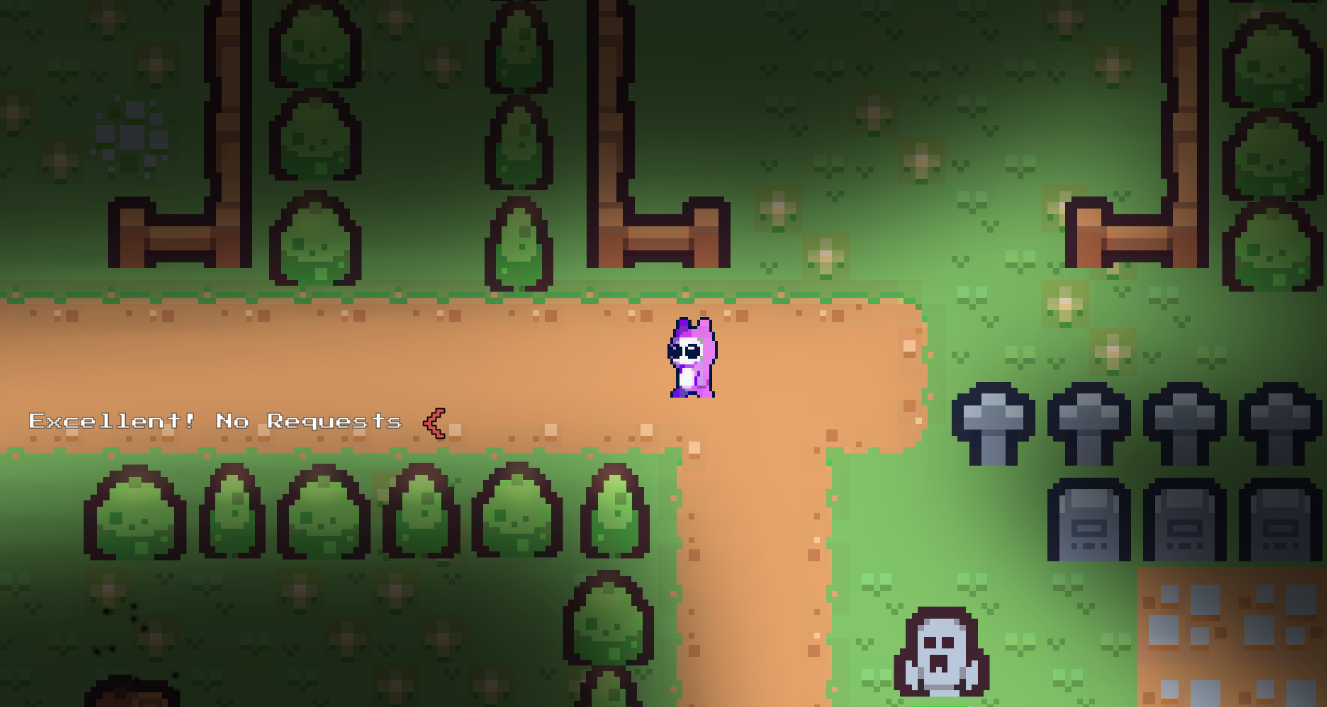
\includegraphics[width=0.85\textwidth]{fog_of_war_effect.png}
\caption{Fog of War effect}
\end{figure}

\subsection{How to Optimize the Fog of War?}

\begin{enumerate}
  \item Cut down the rays. 360 or 180 rays are unnecessary and costly. I tried 15--45 rays --- that was enough, and the experience improved a lot. Below that, uncertainty drops; above that, the cost becomes too heavy for other computers.
  \item Detect the player's movement: when the player stops moving, skip recomputing the fog. I tried computing the shape only once in a while (every 0.2 s) to save CPU, but it failed because the shape could not follow the camera center.
\end{enumerate}

Designer's Note: The fog is a complete system --- not because it's hard to render, but because it turns every step into a choice. I cut the rays from 360 to 30; the players never notice the difference, but the CPU does.

% !TeX root = ../main.tex
% ============================================================
% Chapter 5: Random Dungeon Map
% 说明：本文件由 main.tex 合并进主文档。章节编号 LaTeX 自动生成。
%       内容忠实来自 策划案.docx 原文（英文）。
%       图片：figures/Chapter05_RandomDungeonMap/
%       % TODO: 标记的小节是原文只有标题、没有内容的部分（待补充索引）。
% ============================================================
\section{Random Dungeon Map}

The random dungeon map is the biggest source of uncertainty and the reason players keep coming back to the same dungeon level.

\subsection{Dungeon Map Randomization Principles}

A random dungeon map should follow these principles:

\begin{enumerate}
  \item The road between the exit portal and the spawn point must be accessible.
  \item The terrain must be playable: it needs walls, plenty of open space for walking and fighting, and random obstacles that force players to use strategy.
\end{enumerate}

\subsection{How to Generate a Proper Dungeon Map?}

To generate a proper map, I recommend the steps below --- I have tried them, and they work (The new method is complete and working). This is the design I am most proud of, because it directly supports my core gameplay loop.

\textbf{New Method:}

\begin{enumerate}
  \item Use the cellular automaton algorithm to dig the terrain.
  \item Keep the biggest open area generated by the algorithm. (This is the core optimization step.)
  \item Place the Spawn Point and the Exit Portal randomly inside the open area. Put the spawn point in an open spot, and put the exit as far away as possible, also in an open spot.
  \item Scatter obstacles around the map.
  \item Check that the road between the exit portal and the spawn point stays accessible. If obstacles block the main road, scatter fewer obstacles.
  \item Make sure the Spawn Point and the Exit Portal sit on ground tiles; if not, re-run step 3.
  \item Tile the map and place the prefabs.
\end{enumerate}

Here Shows the effects of the algorithm.

\begin{figure}[htbp]
\centering
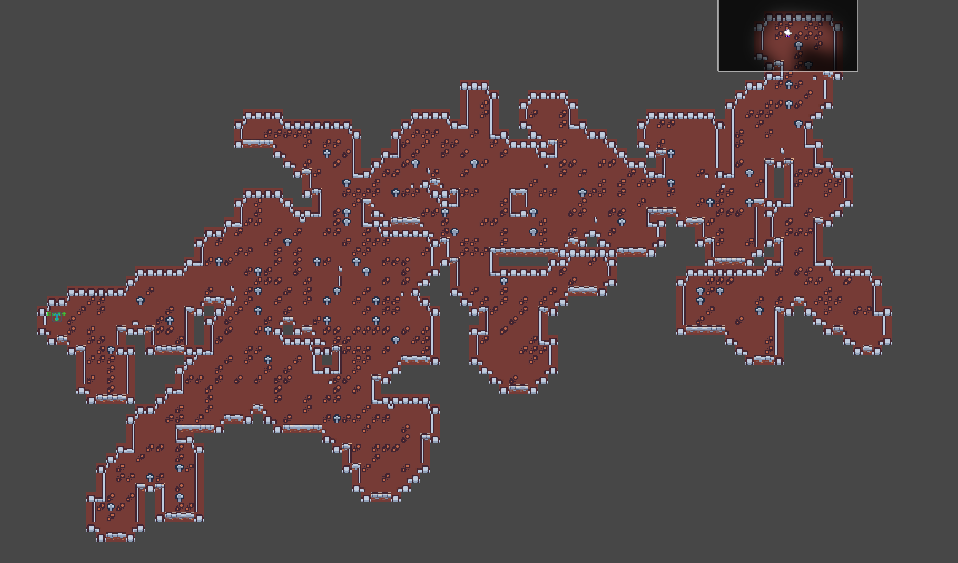
\includegraphics[width=0.85\textwidth]{dungeon_new_method.png}
\caption{New dungeon generation method}
\end{figure}

\textbf{Old Method:}

\begin{enumerate}
  \item Initialize the elements. Set the map scale first: the map is a square with a fixed border. Then place a spawn point and an exit portal in the right spots. In my design, the distance between them should be at least 80\% of the border length, and the exit portal should sit within 95\% of the border length so it never spawns on the border itself.
  \item Guarantee that the road between the exit portal and the spawn point is accessible. The A* algorithm can guarantee a spine road, but it needs optimization --- if we generate the spine road with A* first, the road has no randomization.
  \item Cellular automaton is a good fit for terrain generation. Use it at this step to generate random terrain. Its flaw: it tends to create karst-like terrain with stalactites, and the stalactites make wall generation awkward --- walls look strange when a stalactite has a pointed top.
  \item Cellular automaton may cover the spine road and break the path between the spawn point and the exit portal. This step needs optimization --- it becomes unnecessary when the earlier steps are handled properly.
  \item Once the spine road is generated, use BFS to inject more uncertainty into the map, giving players more adventurous decisions. Because of BFS's nature, it creates many side roads unrelated to the spine road, which can confuse the player.
  \item Dig rooms for the spawn point, the exit portal, combat, and chests. But rooms shouldn't sit right beside the spawn or exit points --- that would reduce the adventure uncertainty.
  \item Scatter random obstacles along the accessible roads. This step has no trick to it, but don't block the essential path with obstacles.
  \item Run an accessibility check --- the road must stay accessible. But this step is redundant if checking is already done in steps 2 and 4. To optimize: check the road once, and prepare a fallback plan in case the road is blocked.
  \item To make wall generation more reliable, cut off the stalactite's pointed top --- otherwise the walls cannot connect properly.
  \item Build the topology of the dungeon map and tile the map. Define each map element as an inside dot, a border dot, or an outside dot. This helps scripts understand tile locations: inside dots render floor, border dots render walls, outside dots render nothing.
  \item Create the exit portal prefab and the enemy spawn area. The enemy spawn area is described in section 5.3.
  \item Send messages to the state machine and the player. When the state machine receives the message, it changes its status to `dungeon'; the player is placed at the spawn point.
  \item Add Collider2D to walls and obstacles.
\end{enumerate}

Tips: the steps above have several defects, so I will reorder them to optimize the pipeline --- using fewer compute resources and generating a more playable dungeon map. The picture below shows version 1.0 of the random dungeon map.

\begin{figure}[htbp]
\centering
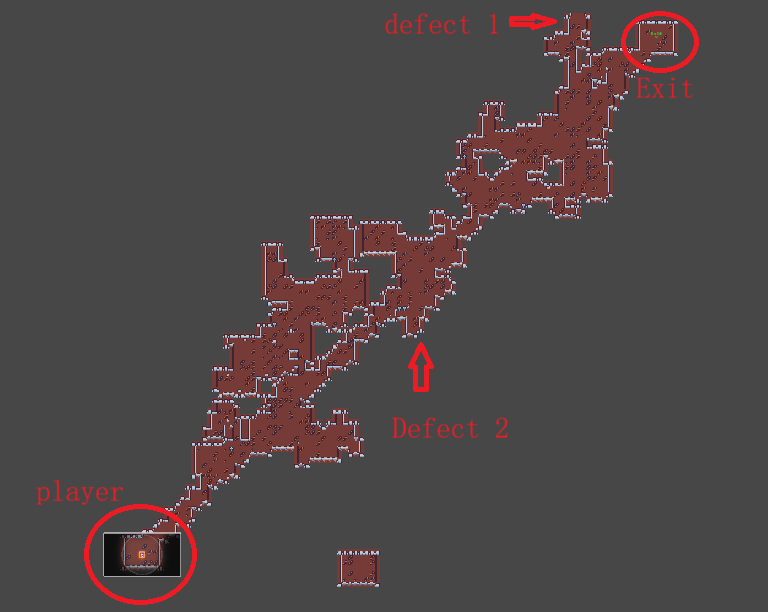
\includegraphics[width=0.85\textwidth]{dungeon_v1_defects.png}
\caption{V1.0 dungeon defects}
\end{figure}

Description of the picture elements:

\begin{enumerate}
  \item Player: the player's spawn point.
  \item Exit: the exit portal's location
  \item Defect 1: the walls don't connect properly, so the player can walk out of the dungeon.
  \item Defect 2: walls appear in the wrong places, making the map look strange.
  \item Defect 3: the exit's location is fixed, so the map doesn't show its randomness.
  \item Defect 4: the open areas are too small, so the player can't fight comfortably in the map.
\end{enumerate}

\subsection{Enemy/Enemy Difficulty Randomize}
% TODO: 原文仅有标题，内容待补充

\subsection{Treasure Randomize}
% TODO: 原文仅有标题，内容待补充

% !TeX root = ../main.tex
% ============================================================
% Chapter 6: Enemy
% 说明：本文件由 main.tex 合并进主文档。章节编号 LaTeX 自动生成。
%       内容忠实来自 策划案.docx 原文（英文）。
%       路径中的反斜杠用 \bs （在 main.tex 中定义为 \textbackslash）。
% ============================================================
\section{Enemy}

\subsection{Module Description}

\par \hspace{1.5em} Divided the system into these modules.

\begin{itemize}
  \item Spawn Enemy: The only express way to contact the spawn message in the each other modules.
  \item Public Config: Store the enemy's static template informations.
  \item Public Script: The module store monster's public behaviour (Core Pipeline).
  \item Special Enemy AI: The module store Special Enemy AI scripts: These scripts modify the core pipeline to change the behaviours.
  \item EnemtMessageBus: The private field message bus provide for Enemy field using.
\end{itemize}

\subsection{System Pipeline}

\begin{enumerate}[label=Step \arabic*:, leftmargin = 5em]
	\item A module send a message to spawn module for generating monsters. The message contains these arguments: Monster Species, numbers, locations.
	\item Enemy Spawn Module subscribes the enemy spawn messages, EnemyPipelineController.cs begins to control the pipeline.
	\item Initialize the correct template data.
	\item Create a Prefab with correct Unity Components, which contains SpriteRenderer, CircleCollider2D/3D, RigidBody2D/3D.
	\item Public Scripts work on the Prefab, add scripts to control the monster's behavoiour.(The Core Pipeline, described at \ref{sec:pipeline})
	\item If the monster carrys special function, then Special Enemy AI's script which correlates to this monster will modify the core pipeline to change properties.
	\item Add the sprites, animations. Transmit the prefab to Enemy Spawn Module.
	\item Enemy Spawn Module send the prefab to renderer.
\end{enumerate}

\subsection{Core Pipeline}\label{sec:pipeline}

\subsubsection{EnemyHealth}

\par \hspace{1.5em} \textbf{Core Data (currentHealth):}

\begin{enumerate}
	\item \texttt {\bs Assets\bs EnemyUnit\bs PublicScript\bs EnemyInit.cs}: Data Initialization Region. Copy the template's data then transmit into the EnemyHealthData.cs to maintain the argument ``currentHealth''.
	\item \texttt {\bs Assets\bs EnemyUnit\bs PublicScript\bs EnemyHealthData.cs}: Maintain the ``currentHealth'' data.
	\item \texttt {\bs Assets\bs EnemyUnit\bs PublicScript\bs Direction.cs}: Recieve and calculate the damage. The only visit tool for ``currentHealth'' in the EnemyHealthData.cs. The submodule's introduction placed in Appendix~\ref{app:c:enemy-movement}.
	\item \texttt {\bs Assets\bs EnemyUnit\bs PublicScript\bs EnemyDeath}: Destory the EnemyPrefab and play the animation.
\end{enumerate}

\par\textbf {Plugs (Relative Path):}

\begin{enumerate}
	\item\texttt {\bs ..\bs Buff\bs EnemyBuffSystem.cs}: The ``DamageBuff'', only control the player providing debuff damage.
	\item\texttt {\bs ..\bs HealthBar}: The enemy's healthbar controller.
	\item\texttt {\bs ..\bs Effects}: The tool to control variable effects, such as hit effects, particle effects.
	\item\texttt {\bs ..\bs Protects}: The tool to protect any kind of inresistible program logic incidents, such as renderer stuck or enemy prefabs stuck into the wall.
	\item\texttt {\bs ..\bs DamagePopUp}: Damage numbers that enemy pop up when player takes damage to the enemy.
\end{enumerate}

\par\textbf {Resources:}
\begin{enumerate}
	\item ``HitParticlePrefab'' controlled by HitParticle (\texttt{\bs ..\bs EnemyHealth\bs Effects\bs HitParticle}) .
	\item ``EnemyPrefab'' is located in the \texttt{\bs Assets\bs Resources\bs Enemy\bs EnemyPrefab}.
	\item ``DamageNumberPrefab'' controlled by DamagePopUp plug(\texttt{\bs ..\bs EnemyHealth\bs DamagePopUp})(Prefab newed by scripts).
\end{enumerate}

\subsubsection{EnemyAttack}

\hspace{1.5em}\textbf{Only use Collider2D to trigger the attack}. When Enemy's Collider2D triggered player's collider, enemy will send a attack data to player's Module `PlayerHealth'.


\subsubsection{EnemyMovement}

\par \hspace{1.5em} Relative Path: \texttt{\bs Assets\bs EnemyUnit\bs PublicScript\bs EnemyMovement}

\par \textbf{Core Data:}

\begin{enumerate}
	\item\texttt{\bs ..\bs EnemyMovementInit.cs}: Initialize the movement data into the EnemyMovementData.cs.
	\item\texttt{\bs ..\bs EnemyMovementData.cs}: Maintainance the movement data which engaged with  'current direction' and 'current speed'.
	\item\texttt{\bs ..\bs EnemySpeedCalculator.cs}: The only port to control the current speed module. The module calculate the final speed and transmit the CurrentSpeed data into EnemyMovementData.cs.
	
	\item\texttt{\bs ..\bs Direction}: The only port to control the current direction module. The module calculate the final direction and transmit the CurrentDirection data into the EnemyMovementData.cs
\end{enumerate}

\par \textbf{Plugs:}
\begin{enumerate}
	\item\texttt{\bs ..\bs EnemyKnockBackApplier}: The plug to control the enemy's knockback.
	\item\texttt{\bs ..\bs PathFindingAlgorithm}: The plug to control the enemy's direction that let enemies along the correct way to catch the player.
\end{enumerate}








% !TeX root = ../main.tex
% ============================================================
% Chapter 7: Version
% 说明：本文件由 main.tex 合并进主文档。章节编号 LaTeX 自动生成。
%       内容忠实来自 策划案.docx 原文（英文）。
%       每个版本记录为一个子节（编号为 7.1 / 7.2 / 7.3，
%       7 是 Version 的章号，由 LaTeX 自动管理）。
% ============================================================
\section{Version}

\subsection{Version 1.0}

Published the primary demo but unfit for playing because the dragging function and sell items function not be inserted. The game code structure, optimizing are not completed and the task, game story has not set. Updated at September 24, 2026.

\subsection{Version 1.1}

Reconstruct the code structure: Applied the new structure to consolidate the structure so as to add new function (Dragging Function \& Sell Items Function) in the game. Optimized the code structure and system pipelines. Completed the Game Design Documentation. Updated at September 30, 2026.

\subsection{Version 1.2}

Added the Dragging Function \& Sell Items Function in the game.


% \appendix 之后，\section 自动编号为 Appendix A / Appendix B / Appendix C（字母编号）
% 注意：\include 会在每个文件前后强制分页，所以 "Appendix" 大标题
% 放在 A_Hierarchy.tex 开头（与 Appendix A 同页），不要放在这里。
\appendix
% !TeX root = ../../main.tex
% ============================================================
% Appendix A: Hierarchy（由 08_appendix.tex 拆分而来）
% 说明：本文件由 main.tex 合并进主文档，且位于 main.tex 的
%       \appendix 之后，因此 \section 会自动编号为 Appendix A。
%       内容忠实来自 策划案.docx 原文（英文）。
%       用 forest 横向树（根在左、向右展开）。
%       【自己加节点】想加子节点：在父节点 [ ] 里加一行 [名字]。
%       例如在 [EnemyPrefab (Example) 的 [ ] 里加 [NewBossAI]。
% ============================================================

% 附录起始页大标题（原在 main.tex，被 \include 的强制分页拆到单独一页；
% 移到本文件开头后与 Appendix A 标题同页）
\begin{center}
{\fontsize{16pt}{45pt}\selectfont\textbf{Appendix}}
\end{center}

\section{Hierarchy}   % 自动显示为 "Appendix A: Hierarchy"

\begin{center}
\begin{forest}
for tree={
  grow=east,
  draw,
  rounded corners=2pt,
  minimum height=2.1em,
  inner xsep=5pt,
  font=\footnotesize\sffamily,
  s sep=4pt,
  l sep=16pt,
  edge={gray, thick},
  parent anchor=east,
  child anchor=west,
  if n children=0{fill=gray!10}{fill=white}
}
[, phantom
  [EventSystem]
  [ParticleSystem]
  [PlayerUnit
    [SpriteRenderer]
    [PlayerAttack [Weapon]]
    [PlayerMovement]
    [PlayerHealth [Plug\_HealthBar]]
    [PlayerStamina [Plug\_StaminaBar]]
  ]
  [EnemyUnit
    [EnemyPrefab (Example)
      [SpriteRenderer]
      [Animation]
      [SpecialAl (If any)]
      [EnemyMovement]
      [EnemyAttack]
      [EnemyHealth]
      [DamagePopUp]
    ]
  ]
]
\end{forest}
\end{center}

% !TeX root = ../../main.tex
% ============================================================
% Appendix B: Player（由 08_appendix.tex 拆分而来）
% 说明：本文件由 main.tex 合并进主文档，且位于 main.tex 的
%       \appendix 之后，因此 \section 会自动编号为 Appendix B。
%       内容忠实来自 策划案.docx 原文（英文）。
%       路径中的反斜杠用 \bs （在 main.tex 中定义为 \textbackslash）。
% ============================================================

\section{Player}   % 自动显示为 "Appendix B: Player"

\subsection{[1] Player Main Config parameters explaination.}

Path: \texttt{\bs Assets\bs PlayerUnit\bs PlayerConfig\bs PlayerConfig.cs}

SubModule: PlayerHealth

\begin{table}[htbp]
\centering
\begin{tabular}{lll}
\toprule
\textbf{Parameters} & \textbf{Function} & \textbf{Data First Read} \\
\midrule
MaxHealth & skim & \texttt{PlayerHealth.cs: cs.44} \\
Defense & skim & \texttt{PlayerHealth.cs: cs.45} \\
InvincibleDuration & Invincible time & \texttt{PlayerHealth.cs: cs.152} \\
\bottomrule
\end{tabular}
\caption{Player main config parameters}
\end{table}

\textbf{Plug (PlayerHealth): PlayerHealthBar}

Path: \texttt{\bs Assets\bs PlayerUnit\bs PlayerHealth\bs Plug\_HealthBar}

Files Introduction:

\begin{itemize}
  \item HealthBarConfig: Control the HealthBar's Animation.
  \item HealthBarUI.DataTransmittion: Read the data.
  \item HealthBarUI.Assembly: Set the UI.
  \item HealthBarUI.Animation: Record the animation types.
  \item HealthBarUI.Display: Display the HealthBar's Animation.
\end{itemize}

\subsection{[2] Player Juice parameters explaination (Play Feelings).}

Path: \texttt{\bs Assets\bs PlayerUnit\bs PlayerConfig\bs PlayerConfig.cs}

% TODO: 原文仅有标题与路径，详细参数待补充

\subsection{[3] Player Messages}

Path: \texttt{\bs Assets\bs PlayerUnit\bs PlayerMessageBus}

Messages SubClass:

\begin{enumerate}
  \item \textbf{PlayerHealth}

  Path: \texttt{\bs Assets\bs PlayerUnit\bs PlayerHealth\bs PlayerHealthMessage.cs}

  Duty: Transmit the CurrentHealth and MaxHealth from PlayHealthCache to Plug\_HealthBar, in order to display the ``CurrentHealth\bs{} MaxHealth'' text.

  Sender: \texttt{\bs Assets\bs PlayerUnit\bs PlayerHealth\bs PlayerHealthCache.cs: cs.53-57.}

  Receiver: \seqsplit{Assets\textbackslash PlayerUnit\textbackslash PlayerHealth\textbackslash Plug\_HealthBar\textbackslash HealthBarUI.DataTransmission: cs.36.}

  \item \textbf{PlayerAttack}

  Path: \texttt{\bs Assets\bs PlayerUnit\bs PlayerAttack\bs PlayerAttackRequestMessage.cs}

  Duty: Transmit three arguments: Direction, PlayerPosition, MousePosition to WeaponSettingsModule.

  Sender: \texttt{\bs Assets\bs PlayerUnit\bs PlayerAttack\bs PlayerAttackAction.cs: cs.65-70.}

  Receiver: \texttt{\bs Assets\bs PlayerUnit\bs PlayerAttack\bs WeaponSettings\bs Iweapon.cs: cs.28.}
\end{enumerate}

% !TeX root = ../../main.tex
% ============================================================
% Appendix C: Enemy（新建，仿照 A_Hierarchy / B_Player 的结构）
% 说明：本文件由 main.tex 合并进主文档，且位于 main.tex 的
%       \appendix 之后，因此 \section 会自动编号为 Appendix C。
%       内容忠实来自 策划案.docx 原文（英文）。
%       路径中的反斜杠用 \bs （在 main.tex 中定义为 \textbackslash）。
% ============================================================

\section{Enemy}   % 自动显示为 "Appendix C: Enemy"
\subsection{EnemyMovement Direction Submodule}\label{app:c:enemy-movement}

\par \hspace{1.5em} Relative Path: \texttt{\bs Assets\bs EnemyUnit\bs PublicScript\bs EnemyMovement\bs Direction}

\begin{enumerate}
	\item Direction Data Maintainance: EnemyDirectorCalculator.cs.
	\item Avoid the obstacle: EnemyAvoidance.cs.
	\item Seperate the enemies movement(do not let enemies engaged together): EnemySeperation.cs.
	\item Decide the state whether to ``Patrol'' or ``Chase''.
	\item Use the BFS algorithm to optimize the chasing algorithm. The algorithm placed in the ``PathFingingAlgorithm'' folder and the algorithm's description placed in \ref{app:c:bfs}.
\end{enumerate}

\subsection{PathFinding Algorithm}\label{app:c:bfs}
\par\hspace{1.5em}The BFS(Broad Field Searching) algorithm will increase the enemy chasing logic, preventing enemy chasing like a noob.
	The BFS algorithm achieved by following steps:
\begin{enumerate}
	\item Scan the whole map into states that combined with 'can walk', 'cannot walk'.
	\item Applied the BFS algorithm into the EnemyMovement's Direction data flow to adjust the moving direction so that enemy will follow the correct path to chase the player.
	\item\textbf{The BFS algorithm's arguments have written in the BFS\_Arguments.cs.}
\end{enumerate}

\end{document}
